\newpage
\section{Tangentes}\label{section:tangentes}
\subsection{Coniques et droites}
\begin{tcolorbox}[colback=cyan!5, colframe=cyan!70!blue, title=Positions relatives d'une droite et une ellipse]
 Soient une ellipse $\mathcal{E}$ et une droite $d$.\\
    \begin{minipage}{0.4\textwidth}
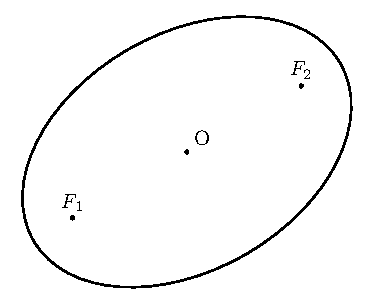
\includegraphics[scale = 0.9]{sections/tikz_standalone/ell_2.pdf}
\end{minipage}
\hfill
    \begin{minipage}{0.6\textwidth}
    \defn{Une droite $d$ est dite \textbf{sécante}\\
     à l'ellipse $\mathcal{E}$ 
lorsqu'elle admet \textbf{2} intersections distinctes avec celle-ci.}
\end{minipage}

\vspace{1.5cm}
    \begin{minipage}{0.4\textwidth}
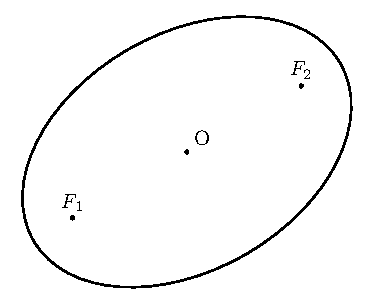
\includegraphics[scale = 0.9]{sections/tikz_standalone/ell_2.pdf}
\end{minipage}
\hfill
    \begin{minipage}{0.6\textwidth}
    \defn{Une droite $d$ est dite \textbf{tangente}\\ à l'ellipse $\mathcal{E}$ 
lorsqu'elle admet exactement \textbf{1} intersection avec celle-ci.}
\end{minipage}

\vspace{1.5cm}
    \begin{minipage}{0.4\textwidth}
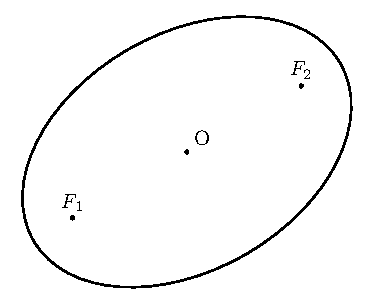
\includegraphics[scale = 0.9]{sections/tikz_standalone/ell_2.pdf}
\end{minipage}
\hfill
    \begin{minipage}{0.6\textwidth}
    \defn{Une droite $d$ est dite \textbf{extérieure}\\ à l'ellipse $\mathcal{E}$ 
lorsqu'elle n'admet \textbf{aucune} intersection avec celle-ci.}
\end{minipage}
\end{tcolorbox}
%\subsection{Tangente à une ellipse}
%\subsection{Tangente à une parabole}
%\subsection{Tangente à une hyperbole}
\newpage
\begin{tcolorbox}[colback=cyan!5, colframe=cyan!70!blue, title=Positions relatives d'une droite et une hyperbole]
Soient une hyperbole $\mathcal{H}$ et une droite $d$ \textbf{non parallèle aux asymptotes de l'hyperbole}.\\
    \begin{minipage}{0.4\textwidth}
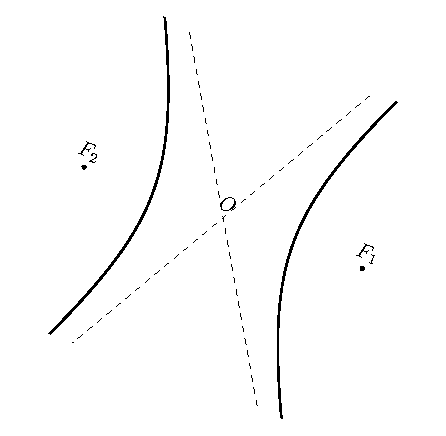
\includegraphics[scale = 0.9]{sections/tikz_standalone/hyp_15.pdf}
\end{minipage}
\hfill
    \begin{minipage}{0.6\textwidth}
    \defn{Une droite $d$ non parallèle aux asymptotes de l'hyperbole $\mathcal{H}$ est dite \textbf{sécante}\\
     à celle-ci 
lorsqu'elle admet \textbf{2} intersections distinctes avec celle-ci.}
\end{minipage}

\vspace{1.5cm}
    \begin{minipage}{0.4\textwidth}
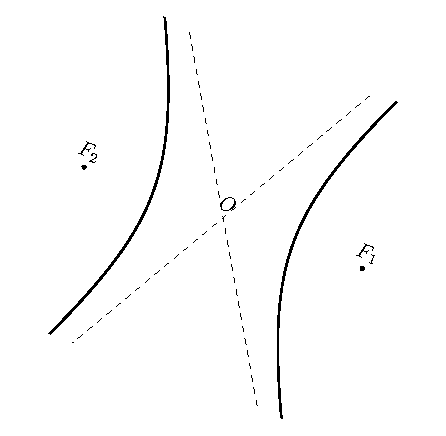
\includegraphics[scale = 0.9]{sections/tikz_standalone/hyp_15.pdf}
\end{minipage}
\hfill
    \begin{minipage}{0.6\textwidth}
    \defn{Une droite $d$ non parallèle aux asymptotes de l'hyperbole $\mathcal{H}$ est dite 
    \textbf{tangente}\\ à celle-ci 
lorsqu'elle admet exactement \textbf{1} intersection avec celle-ci.}
\end{minipage}

\vspace{1.5cm}
    \begin{minipage}{0.4\textwidth}
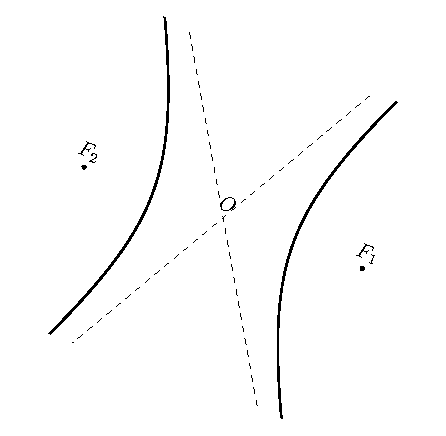
\includegraphics[scale = 0.9]{sections/tikz_standalone/hyp_15.pdf}
\end{minipage}
\hfill
    \begin{minipage}{0.6\textwidth}
    \defn{Une droite $d$ non parallèle aux asymptotes de l'hyperbole $\mathcal{H}$ 
    est dite \textbf{extérieure}\\ à celle-ci 
lorsqu'elle n'admet \textbf{aucune} intersection avec celle-ci.}
\end{minipage}
\end{tcolorbox}
\newpage

\begin{tcolorbox}[colback=cyan!5, colframe=cyan!70!blue, title=Positions relatives d'une droite et une hyperbole]
Soient une hyperbole $\mathcal{H}$ et une droite $d$ \textbf{parallèle à une asymptote de l'hyperbole et distincte de celle-ci}.\\
    \begin{minipage}{0.4\textwidth}
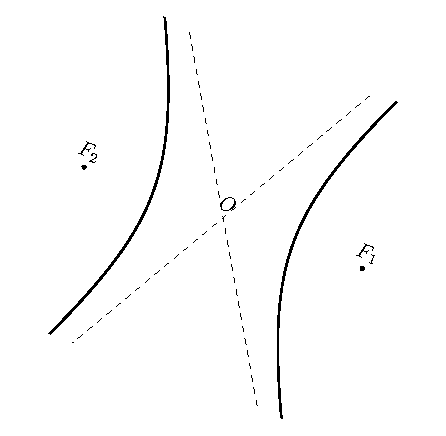
\includegraphics[scale = 0.9]{sections/tikz_standalone/hyp_15.pdf}
\end{minipage}
\hfill
    \begin{minipage}{0.6\textwidth}
    \prop{Une droite $d$ parallèle à une asymptote de l'hyperbole $\mathcal{H}$ 
    et distincte de celle-ci a exactement \textbf{1} intersection avec l'hyperbole.}
\end{minipage}

\vspace{1.5cm}
Soient une hyperbole $\mathcal{H}$ et une droite $d$ étant \textbf{une asymptote de l'hyperbole}.\\

    \begin{minipage}{0.4\textwidth}
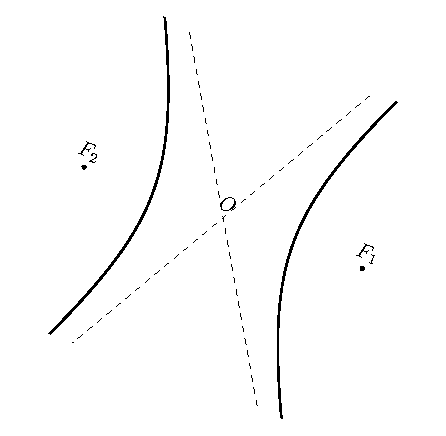
\includegraphics[scale = 0.9]{sections/tikz_standalone/hyp_15.pdf}
\end{minipage}
\hfill
    \begin{minipage}{0.6\textwidth}
    \prop{Une droite $d$ étant une asymptote de l'hyperbole $\mathcal{H}$ n'a \textbf{aucune} intersection avec celle-ci.}
\end{minipage}




\end{tcolorbox}
\newpage

\begin{tcolorbox}[colback=cyan!5, colframe=cyan!70!blue, title=Positions relatives d'une droite et une parabole]
Soient une parabole $\mathcal{P}$ et une droite $d$ \textbf{non parallèle à l'axe de la parabole}.\\
    \begin{minipage}{0.4\textwidth}
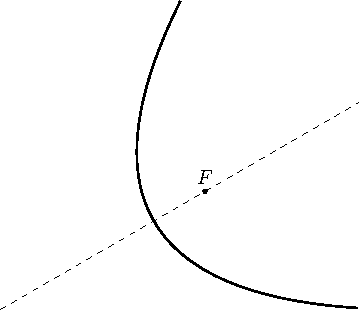
\includegraphics[scale = 0.9]{sections/tikz_standalone/para_13.pdf}
\end{minipage}
\hfill
    \begin{minipage}{0.6\textwidth}
    \defn{Une droite $d$ non parallèle à l'axe de la parabole $\mathcal{P}$ est dite \textbf{sécante}\\
     à celle-ci 
lorsqu'elle admet \textbf{2} intersections distinctes avec celle-ci.}
\end{minipage}

\vspace{1.5cm}
    \begin{minipage}{0.4\textwidth}
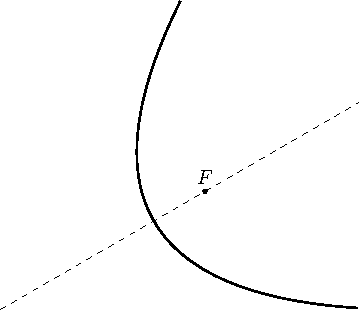
\includegraphics[scale = 0.9]{sections/tikz_standalone/para_13.pdf}
\end{minipage}
\hfill
    \begin{minipage}{0.6\textwidth}
    \defn{Une droite $d$ non parallèle à l'axe de la parabole $\mathcal{P}$ est dite 
    \textbf{tangente}\\ à celle-ci 
lorsqu'elle admet exactement \textbf{1} intersection avec celle-ci.}
\end{minipage}

\vspace{1.5cm}
    \begin{minipage}{0.4\textwidth}
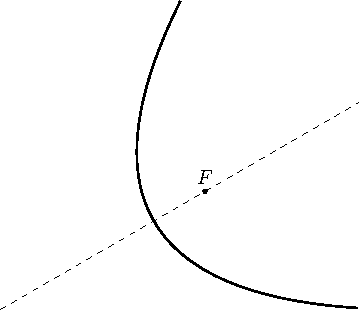
\includegraphics[scale = 0.9]{sections/tikz_standalone/para_13.pdf}
\end{minipage}
\hfill
    \begin{minipage}{0.6\textwidth}
    \defn{Une droite $d$ non parallèle à l'axe de la parabole $\mathcal{P}$ 
    est dite \textbf{extérieure}\\ à celle-ci 
lorsqu'elle n'admet \textbf{aucune} intersection avec celle-ci.}
\end{minipage}
\vspace{1.5cm}

Soient une parabole $\mathcal{P}$ et une droite $d$ \textbf{parallèle à l'axe de la parabole}.\\
\begin{minipage}{0.4\textwidth}
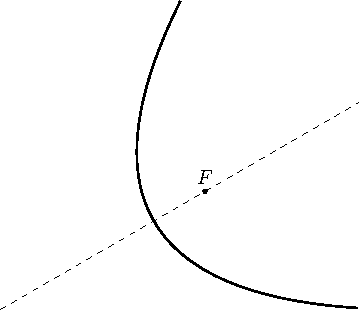
\includegraphics[scale = 0.9]{sections/tikz_standalone/para_13.pdf}
\end{minipage}
\hfill
    \begin{minipage}{0.6\textwidth}
    \prop{Une droite $d$ parallèle à l'axe de la parabole $\mathcal{P}$ admet exactement 
    \textbf{1} intersection avec celle-ci.}
\end{minipage}

\end{tcolorbox}

\newpage

\subsection{Intersection entre une conique $\mathcal{C}$ et une droite $d$}

Nous savons qu'un système de 2 équations décrit le lieu des points vérifiant les 2 équations à la fois.
Les intersections entre une conique et une droite sont donc données par le système composé 
de l'équation de la conique et de l'équation de la droite.

Il suffit donc de résoudre le système d'équations pour trouver les points d'intersections (s'ils existent).

\exth{Calculer les coordonnées des points d'intersections de 
$\mathcal{E} \equiv x^2 + 4 y^2 = 4$ et de la droite $d\equiv y = x-1$.}
\newpage
\subsection{Coniques et droites tangentes}

\subsubsection{Droite tangente à une conique en un point de la conique $\mathcal{C}$}

\begin{minipage}{0.3\textwidth}
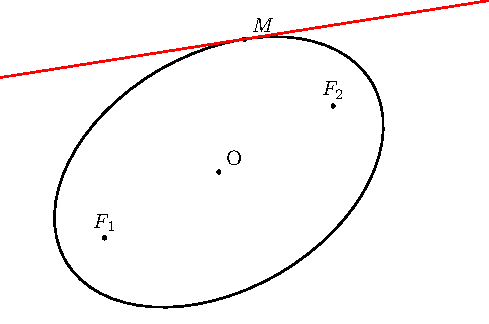
\includegraphics[scale = 0.6]{sections/tikz_standalone/ell_15.pdf}
\end{minipage}
\hfill
\begin{minipage}{0.3\textwidth}
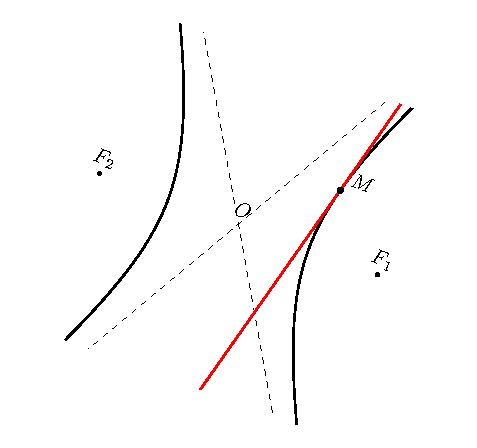
\includegraphics[scale = 0.6]{sections/tikz_standalone/hyp_16.pdf}
\end{minipage}
\hfill
\begin{minipage}{0.3\textwidth}
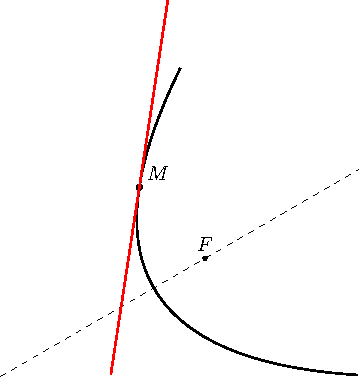
\includegraphics[scale = 0.6]{sections/tikz_standalone/para_14.pdf}
\end{minipage}
\hfill

La tangente au point $M(r,s) \in \mathcal{C}$ est une droite de la forme $t_M \equiv y = mx+q$.\\
Nous cherchons alors la pente $m$ et l'ordonnée à l'origine $q$ de cette tangente.\\

Pour trouver $q$, comme $M$ est un point de la tangente, $M$ vérifie l'équation de la tangente, 
c'est-à-dire $s = mr + q$. On a alors $q = s - mr$.\\

La droite tangente cherchée est alors de la forme $t_M \equiv y-s=m(x-r)$.\\

Ensuite pour trouver la pente $m$ de la tangente, nous nous intéressons aux dérivées premières que 
nous avions calculées précédemment dans les études graphiques des coniques.
Dans nos études graphiques des coniques centrées en $(0,0)$, 
nous avions décomposé les coniques en 2 fonctions : une partie supérieure $f_1(x)$ et une partie inférieure $f_2(x)$ .\\
Les expressions des dérivées premières en un point $M(r,s)$ de la courbe sont reprises ci-dessous.

\subsubsubsection{Ellipse}
\begin{center}
\renewcommand{\arraystretch}{2} % increase row height
\begin{tabular}{c|c|c|c|c}
\hline
 & Equation cartésienne & Dérivée première& Dérivée première& Dérivée première\\
 &  & \textbf{$s>0$} & \textbf{$s=0$} & \textbf{$s<0$} \\
\hline
Ellipse & $ \dfrac{x^2}{a^2} + \dfrac{y^2}{b^2} = 1 $ & $f_1'(r) = -\dfrac{b r}{a \sqrt{a^2-r^2}}$ & 
$\infty$ & $f_2'(r) = \dfrac{b r}{a \sqrt{a^2-r^2}}$ \\
 & $\left(\dfrac{r^2}{a^2} + \dfrac{s^2}{b^2} = 1 \right)$ & $ = -\dfrac{b^2 r}{a^2 s}$ & & $ = -\dfrac{b^2 r}{a^2 s}$ \\
\hline
\end{tabular}
\end{center}

On obtient alors l'équation de la tangente en un point $M(r,s)$ d'une ellipse :
\[t_M \equiv y-s = -\dfrac{b^2 r}{a^2 s} (x-r)\]
ou encore :
\[t_M \equiv b^2rx + a^2sy - a^2b^2=0
\]


\newpage
\subsubsubsection{Hyperbole}
\begin{center}
\renewcommand{\arraystretch}{2} % increase row height
\begin{tabular}{c|c|c|c|c}
\hline
 & Equation cartésienne & Dérivée première& Dérivée première& Dérivée première\\
 &  & \textbf{$s>0$} & \textbf{$s=0$} & \textbf{$s<0$} \\
\hline
Hyperbole & $\dfrac{x^2}{a^2} - \dfrac{y^2}{b^2} = 1$ & $f_1'(r) = \dfrac{b r}{a \sqrt{r^2 - a^2}}$ & $\infty$ & $f_2'(r) = -\dfrac{b r}{a \sqrt{r^2 - a^2}}$ \\
 &  $\left(\dfrac{r^2}{a^2} - \dfrac{s^2}{b^2} = 1\right)$ & $= \dfrac{b^2 r}{a^2 s}$ & & $ = \dfrac{b^2 r}{a^2 s}$ \\
\hline
\end{tabular}
\end{center}

On obtient alors l'équation de la tangente en un point $M(r,s)$ d'une hyperbole :
\[t_M \equiv y-s = \dfrac{b^2 r}{a^2 s} (x-r)\]
ou encore :
\[t_M \equiv b^2rx - a^2sy - a^2b^2=0
\]

\subsubsubsection{Parabole}
\begin{center}
\renewcommand{\arraystretch}{2} % increase row height
\begin{tabular}{c|c|c|c|c}
\hline
 & Equation cartésienne & Dérivée première& Dérivée première& Dérivée première\\
 &  & \textbf{$s>0$} & \textbf{$s=0$} & \textbf{$s<0$} \\
\hline
Parabole & $y^2 = 2px$ & $f_1'(x) = \dfrac{p}{\sqrt{2px}}$ & $\infty$ & $f_2'(x) = -\dfrac{p}{\sqrt{2px}}$ \\
 & $\left(s^2 = 2pr\right)$ & $= \dfrac{p}{s}$ &  & $= \dfrac{p}{s}$ \\

\hline
\end{tabular}
\end{center}

On obtient alors l'équation de la tangente en un point $M(r,s)$ d'une parabole :
\[t_M \equiv y-s = \dfrac{p}{s} (x-r)\]
ou encore :
\[t_M \equiv sy = px +pr 
\]

\newpage

\subsubsection{Droite tangente à une conique issue d'un point hors de la conique $\mathcal{C}$}
\begin{minipage}{0.3\textwidth}
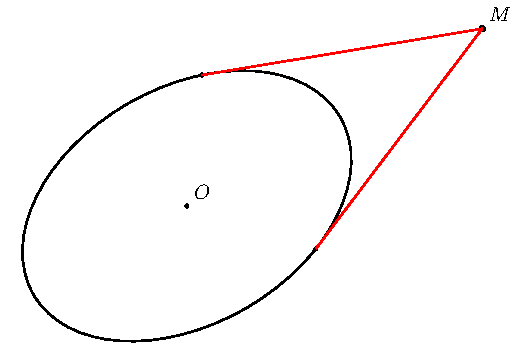
\includegraphics[scale = 0.6]{sections/tikz_standalone/ell_16.pdf}
\end{minipage}
\hfill
\begin{minipage}{0.3\textwidth}
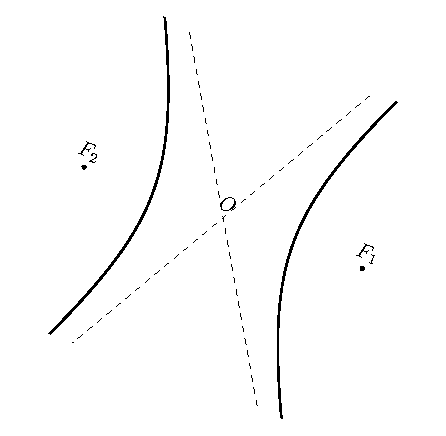
\includegraphics[scale = 0.6]{sections/tikz_standalone/hyp_15.pdf}
\end{minipage}
\hfill
\begin{minipage}{0.3\textwidth}
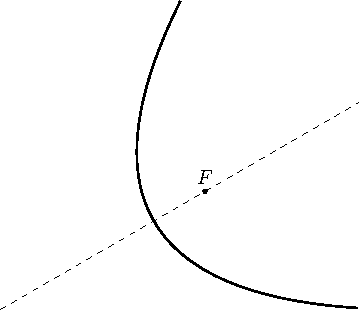
\includegraphics[scale = 0.6]{sections/tikz_standalone/para_13.pdf}
\end{minipage}
\hfill

Les tangentes issues du point $M(r,s) \notin \mathcal{C}$ sont des droites de la forme $t_M \equiv y = mx+q$.\\
Nous cherchons la pente $m$ et l'ordonnée à l'origine $q$ de ces tangentes.\\

Pour trouver $q$, comme $M$ est un point de la tangente, $M$ vérifie l'équation de la tangente, 
c'est-à-dire $s = mr + q$. On a encore une fois $q = s - mr$.\\

Les droites tangentes cherchées sont alors de la forme $t_M \equiv y-s=m(x-r)$.\\
Nous cherchons alors toutes les valeurs de $m$ telles 
qu'il n'y a qu'une intersection entre la droite $t_M$ et la conique.\\
Attention, on peut avoir une seule intersection et avoir une droite non tangente 
(certains cas de l'hyperbole et de la parabole), il faudra rejeter ces solutions.

\exth{Trouver les équations cartésiennes des tangentes à l'ellipse $\mathcal{E} \equiv 4x^2 + y^2 = 4$ issues du point $M(0,3)$}



\newpage
\exth{Trouver les équations cartésiennes des tangentes à l'hyperbole \\
$\mathcal{H} \equiv 9x^2 - 16y^2 = -144$ issues du point $M(4,3)$}

\vspace{11cm}
\subsubsection{Droite tangente à une conique $\mathcal{C}$ avec une pente $m$ donnée}
\begin{minipage}{0.3\textwidth}
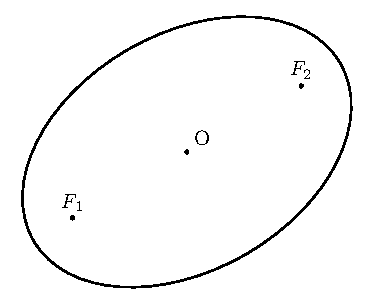
\includegraphics[scale = 0.6]{sections/tikz_standalone/ell_2.pdf}
\end{minipage}
\hfill
\begin{minipage}{0.3\textwidth}
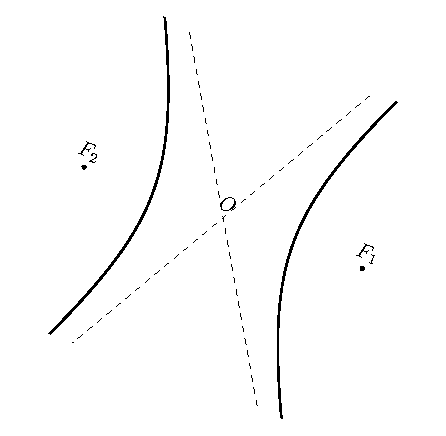
\includegraphics[scale = 0.6]{sections/tikz_standalone/hyp_15.pdf}
\end{minipage}
\hfill
\begin{minipage}{0.3\textwidth}
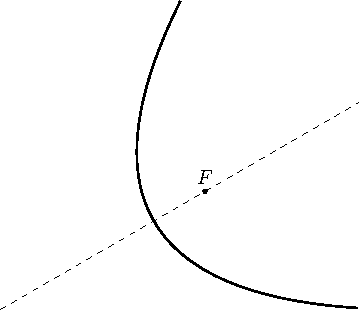
\includegraphics[scale = 0.6]{sections/tikz_standalone/para_13.pdf}
\end{minipage}
\hfill

Les tangentes dont on connait la pente $m$ sont des droites de la forme $t_M \equiv y = mx+q$.\\
Nous cherchons toutes les valeurs de $q$ telles 
qu'il n'y a qu'une intersection entre la droite $t_M$ et la conique.\\

\exth{Trouver les équations cartésiennes des tangentes à la parabole \\
$\mathcal{P} \equiv y^2 = 4x$ avec un coefficient angulaire $m = 2$.}
\newpage
\null
\newpage